\chapter{Θεωρητικό υπόβαθρο}

Ένα απλό πολύγωνο είναι η περιοχή του επιπέδου που περικλείεται από ένα πεπερασμένο σύνολο ευθυγράμμων τμημάτων τα οποία σχηματίζουν μία κλειστή τεθλασμένη γραμμή. Τα $n$ ευθύγραμμα τμήματα αυτής της τμηματικώς γραμμικής καμπύλης αποτελούν τις ακμές του πολυγώνου και, σε συνδυασμό με τις $n$ κορυφές του, ορίζουν ένα πολυγωνικό πλέγμα ή μία πολυγωνική επιφάνεια. Στην πρώτη περίπτωση, σημεία του σχήματος θεωρούνται όσα σημεία ανήκουν στις ακμές, ενώ στη δεύτερη περίπτωση χρειάζεται ένας έλεγχος εσωτερικότητας των σημείων για να διαπιστωθεί αν αυτά ανήκουν στην επιφάνεια που ορίζεται από τις ακμές (Δρακόπουλος, 2021? Μουστάκας κ.ά., 2015? Παληός, 2021).

\section{Έλεγχος εσωτερικού σημείου}
Σύμφωνα με το θεώρημα καμπύλης \textlatin{Jordan (Jordan Curve Theorem)}, μία συνεχής, απλή, κλειστή και επίπεδη καμπύλη χωρίζει το επίπεδο σε δύο περιοχές, την εσωτερική (\textlatin{interior}) και την εξωτερική (\textlatin{exterior}) (Δρακόπουλος, 2021? Παληός, 2021). Οι αλγόριθμοι χάραξης πολυγώνων βασίζονται στον έλεγχο εσωτερικότητας κάθε σημείου του πολυγώνου. Οι κύριες μέθοδοι ελέγχου εσωτερικού σημείου είναι ο έλεγχος πλήθους συστροφών (\textlatin{winding number test}) και ο έλεγχος ισοτιμίας (\textlatin{parity test}). Συγκεκριμένα, ο δεύτερος έλεγχος πραγματοποιείται με τον σχεδιασμό ημιευθείας από το εικονοστοιχείο $p$ και την αρίθμηση του πλήθους των τομών της ημιευθείας με την περίμετρο του πολυγώνου $P$. Εφόσον ο αριθμός αυτός είναι περιττός, το $p$ είναι εσωτερικό του $P$; διαφορετικά, το $p$ είναι εξωτερικό του $P$ (Δρακόπουλος, 2021? Μουστάκας κ.ά., 2015).

\section{Ψηφιδόξυση πολυγώνου}
Ο βασικός αλγόριθμος ψηφιδόξυσης πολυγώνου βασίζεται στον έλεγχο ισοτιμίας. Ο αλγόριθμος υπολογίζει τις τομές $I(x, y)$ κάθε ακμής με όλες τις γραμμές διερεύνησης και τις αποθηκεύει σε μία κατάσταση, όπου πραγματοποείται η ταξινόμησή τους με κύριο κλειδί τη συντεταγμένη $y$ και δευτερεύον κλειδί τη συντεταγμένη $x$. Τέλος, εξάγει ζεύγη διαδοχικών σημείων τομής, τα οποία ονομάζονται εκτάματα και αντιπροσωπεύουν τις σειρές εικονοστοιχείων εσωτερικές του πολυγώνου (Δρακόπουλος, 2021? Σπύρου, 2019). \par

Ο παραπάνω αλγόριθμος δεν αποτελεί τη βέλτιστη μέθοδο ψηφιδόξυσης πολυγώνου, δεδομένου ότι η εύρεση του σημείου τομής είναι μία υπολογιστικά ακριβή πράξη. Μία αποδοτικότερη μέθοδος είναι ο αλγόριθμος χάραξης πολυγώνων κατά γραμμές διερεύνησης, ο οποίος εκμεταλλεύεται τη συνάφεια των γραμμών διερεύνησης και τη συνάφεια των ακμών που τέμνουν διαδοχικές γραμμές σάρωσης, και αποθηκεύει τις τομές της εκάστοτε γραμμής διερεύνησης σε μία δομή με τις ακμές του πολυγώνου. Ο αλγόριθμος χάραξης πολυγώνων κατά γραμμές διερεύνησης, η μέθοδος χάραξης με Πίνακα Ακμών και ο αλγόριθμος κρίσιμων σημείων, περιγράφονται αναλυτικά από τους Δρακόπουλο (2021, σ. 141-150), Μουστάκα και συνεργάτες (2015, σ. 40-42), και Σπύρου (2019, σ. 50-58).

\subsection{Αλγόριθμος χάραξης τριγώνου}
Όπως αναφέρθηκε στην \textbf{Εισαγωγή}, το τρίγωνο είναι το απλούστερο, επίπεδο, κυρτό πολύγωνο. Ένας τρόπος καθορισμού των εικονοστοιχείων τα οποία καλύπτουν ένα τρίγωνο είναι η εκτέλεση ελέγχου εσωτερικού σημείου σε όλα τα εικονοστοιχεία ευρισκόμενα εντός του περιβάλλοντος κυτίου του τριγώνου, δηλαδή του συνόλου έκτασης συντεταγμένων του τριγώνου, το οποίο περιέχει τις ελάχιστες και μέγιστες τιμές $x$, $y$ και $z$\footnote{Η πληροφορία υπεύθυνη για το χρώμα του εικονοστοιχείου αποθηκεύεται στη συντεταγμένη $z$.} του αντικειμένου (Δρακόπουλος, 2021? Σπύρου, 2019).

\subsection{Αλγόριθμος χάραξης κυρτού πολυγώνου}
Η χάραξη κυρτών πολυγώνων απαιτεί την υλοποίηση ενός παρόμοιου αλγορίθμου, εφόσον έχει πραγματοποιηθεί έλεγχος κυρτότητας των εν λόγω πολυγώνων. Μία χρήσιμη γεωμετρική δομή η οποία δύναται να διευκολύνει τον έλεγχο κυρτότητας πολυγώνων είναι το κυρτό περίβλημα (\textlatin{convex hull}). Το κυρτό περίβλημα ή κέλυφος ενός συνόλου σημείων $S$ στο επίπεδο ορίζεται ως το μικρότερο κυρτό πολύγωνο $Ρ$ που περικλείει το $S$, δηλαδή η τεθλασμένη γραμμή η οποία περικλείει πλήρως το σύνολο $S$, ώστε να εξαλείφονται οι κοιλότητες της γραμμής (Παληός, 2021, σ. 2? \textlatin{Sharma}, 2018). \par

\begin{figure}[h]
\centering
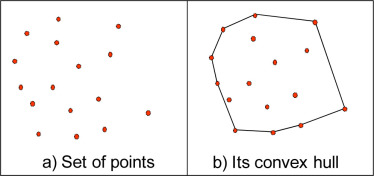
\includegraphics[width=0.5\textwidth]{images/convexhull}
\caption{Κυρτό περίβλημα ενός συνόλου σημείων}
\end{figure}

Οι πιο γνωστοί αλγόριθμοι εύρεσης του κυρτού περιβλήματος ενός πεπερασμένου συνόλου σημείων στο επίπεδο είναι ο αλγόριθμος σάρωσης του \textlatin{Graham (Graham’s scan}), ο αλγόριθμος περιτυλίγματος (\textlatin{Gift wrapping algorithm}) και ο αλγόριθμος του \textlatin{Chan},  όπως αυτοί περιγράφονται αναλυτικά από τους \textlatin{Graham (1972), Jarvis (1973)} και \textlatin{Chan (1996)} αντίστοιχα. Ο πρώτος αλγόριθμος υπολογίζει το κυρτό περίβλημα σε χρόνο $O(n \log n)$, ενώ ο δεύτερος έχει χρονική πολυπλοκότητα $O(nh)$, όπου $n$ το πλήθος των σημείων του επιπέδου και $h$ το πλήθος των απαιτούμενων επαναλήψεων για την εύρεση του κυρτού περιβλήματος. Ο τρίτος αλγόριθμος συνδυάζει τους δύο προηγούμενους ώστε να εξασφαλίσει μία χρονική πολυπλοκότητα $O(n \log h)$ (Κωστόπουλος, 2013).

\subsubsection{Αλγόριθμος περιτυλίγματος}
Δεδομένης της χρονικής πολυπλοκότητας του καθενός εκ των τριών προαναφερθέντων αλγορίθμων, ο αλγόριθμος περιτυλίγματος είναι ο βέλτιστος αλγόριθμος για την εύρεση του κυρτού περιβλήματος ενός περιορισμένου πλήθους σημείων $n$, ενώ αποτελεί χείριστη επιλογή όταν πρόκειται για ένα σημαντικό σύνολο σημείων $S$. \par

Η διαδικασία υπολογισμού ενός κυρτού περιβλήματος είναι ευκόλως ερμηνεύσιμη. Θέτοντας ως πρώτο σημείο $p_1$ του συνόλου $S$ το αριστερότερο σημείο, δηλαδή το σημείο ελάχιστης τιμής $x$, εντοπίζουμε το επόμενο σημείο $p_2$ το οποίο έχει ελάχιστη πολική γωνία $\geq 0$ του $p_1$. Ομοίως συγκρίνουμε σε χρόνο $O(n)$ τις πολικές γωνίες όλων των σημείων $n$ σε σχέση με το σημείο $p_i$ θεωρούμενο το κέντρο των πολικών συντεταγμένων, και επαναλαμβάνουμε τη διαδικασία $h$ φορές ωσότου $p_h=p_1$. Εν ολίγοις, ο εσωτερικός βρόχος ελέγχει κάθε σημείο του συνόλου $S$ και ο εξωτερικός βρόχος επαναλαμβάνεται για κάθε σημείο του περιβλήματος. Ως εκ τούτου, ο συνολικός χρόνος εκτέλεσης είναι $O(nh)$ και εξαρτάται από το μέγεθος της εξόδου, δηλαδή πρόκειται για έναν αλγόριθμο ευαίσθητο εξόδου\footnote{Αλγόριθμος ευαίσθητος εξόδου χαρακτηρίζεται ο αλγόριθμος του οποίου η χρονική πολυπλοκότητα εξαρτάται από το μέγεθος εξόδου του περιβλήματος.} (Κωστόπουλος, 2013? \textlatin{Jarvis, 1973}). \par

\pagebreak